Standards and technologies for web applications are being rapidly developed, and the boundaries for what is possible to achieve in a web application is being continously pushed by browser vendors and standards groups. Of relevance to Rymd, the Web Real-Time Communications (WebRTC) protocol \cite{WebRTC:Online} has become usable for arbitrary data streams in major browsers in 2014. Also of relevance, the still unfinalized Web Crypto API \cite{WebCrypto:Online} is currently available in an experimental stage in recent months at the time of this writing. The goals of Rymd has thus become technically viable in a web environment as of very recently.

Furthermore, there is currently a lot of work underway in the field of distributed secret communication. Notable projects that share similar ideas or have inspired Rymd are mentioned under section~\ref{sec:similar}. Also worth noting is the new field of cryptocurrencies, which work by distributing a cryptographically based ledger over an entire network. The first and most well-known is Bitcoin \cite{Bitcoin:Online}, but there are also subsequent currencies that extend the original idea beyond that of a traditional currency to a system that can be used for a wide range of applications. The first worth noting is Namecoin \cite{Namecoin:Online}, which adds a global and secure key-value store. Another interesting initiative is Ethereum \cite{Ethereum:Online}, a cryptocurrency with contracts that not only allow storage of arbitrary data in the blockchain, but can also be scripted with a Turing complete programming language and can therefore be used to implement arbitrary systems. A system like Ethereum could be very interesting to explore for a project like Rymd, but it is still in such an early stage that it is deemed too unstable to be useful at this point. Namecoin is currently considered a good candidate for key distribution.

Keybase \cite{Keybase:Online} is another recent initiative that intends to solve the distribution of public keys. It is essentially a HTTP-interface that maps keys to identities. While commandable, it again raises the issue of centralized storage. Systems relying on Keybase put a lot of trust on the availability and integrity of their service.

% TODO Johan Data Storage

\section{Data storage}
\label{sec:datastorage}

Storage of data is, suffice to say, crucial for any file sharing system. Since the data store was to be used by several parts of the application the demands for the module's interface had to be as general as possible, adhering to a standard CRUD\footnote{Create–Read–Update–Delete} interface, including methods for creating, fetching, updating and deleting records in the store.

There are essentially four alternatives for persisting data on the client:

\begin{itemize}
\item LocalStorage
\item IndexedDB
\item WebSQL
\item FileSystem API
\end{itemize}

LocalStorage is included in the HTML5 WebStorage specification \cite{WebStorage:Online}, and is a basic key-value store with a simplistic API. It is supported across all major browsers and has a maximum storage limit of 5 megabytes. The latter was a deal-breaker, since the product would have to support larger files than could possibly fit into that space. LocalStorage further does not support complex structures and indexing, and storing different data types is complex and needs manual serialization and deserialization. Thus this solution was rejected at once.

IndexedDB and WebSQL are both client side databases and more sophisticated storage solutions than LocalStorage. WebSQL is supported by Google Chrome, Apple Safari (desktop and iOS), Opera and Android. The specification is not longer maintained by W3C \cite{WebSQL:Online}, and will probably be deprecated on all browsers in the future. IndexedDB is supported by all major browsers except for Safari (desktop and iOS), and is a Candidate Recommendation by W3C \cite{IndexedDB:Online}. Arbitrary types of data can be stored in the database, such as strings, numbers, Javascript objects, and raw binary data.

The FileSystem API is a collection of methods for reading and writing to a sandboxed filesystem from a browser with client Javascript code. It is a very early standard, and is currently only supported by Google Chrome and Opera, and has the status of Working Draft by W3C \cite{FileSystem:Online}. While FileSystem has good performance for larger files and a well-performing asynchronous API, it lacks support for indexing and search. Mozilla seems to have no plans on implementing FileSystem in Firefox \cite{MozillaFileSystem:Online}.

All of the mentioned technologies are sandboxed: the data is tied to a single origin (\emph{http://test.domain.com} for instance). All future access to the data must come from that domain (this includes the protocol and port number as well). The browsers also limits the maximum allowed storage size – the quota. The quota is different for each storage mechanism, and the browser typically asks the user with a dialog if they want to let the app exceed the quota.

\begin{table}
    \begin{tabular}{|l|l|l|l|l|}
    \hline
                       & IndexedDB & WebSQL & File System & LocalStorage \\ \hline
    Google Chrome 34               & Yes       & Yes    & Yes  & Yes                      \\ \hline
    Mozilla Firefox 29             & Yes       & \cellcolor{red}No  & \cellcolor{red}No   & Yes                        \\ \hline
    Apple Safari 7                & \cellcolor{red}No        & Yes  & \cellcolor{red}No    & Yes                        \\ \hline
    Opera 20                       & Yes       & Yes    & Yes  & Yes                      \\ \hline
    Microsoft Internet Explorer 11 & Yes       & \cellcolor{red}No  & \cellcolor{red}No   & Yes                        \\ \hline
    \end{tabular}
    \caption {Browser support for selected HTML5 APIs at the time of writing}
\end{table}

The conclusion was to use IndexedDB for persisted resource storage. It was chosen because of its support by Google Chrome, Internet Explorer and Firefox, and due to the fact that its actively maintained (while WebSQL is not). Users of the Safari browser will not be able to utilize the product, but in respect to the project's overall direction in regards to experimental technologies, this is negligible.

\subsection{IndexedDB}
\label{sec:indexeddb}
% More stuff here: http://www.cms.livjm.ac.uk/pgnet2012/Proceedings/Papers/1569607913.pdf
The IndexedDB is a transactional, indexed client side database capable of storing different types of data structures with an asynchronous API. IndexedDB is actively developed and implemented in the latest versions of Mozilla Firefox, Google Chrome, Microsoft Internet Explorer and Opera: its specification is a Candidate Recommendation by the W3C, as of July 2013\cite{IndexedDB:Online}:

\begin{quote}
This document defines APIs for a database of records holding simple values and hierarchical objects. Each record consists of a key and some value. Moreover, the database maintains indexes over records it stores. An application developer directly uses an API to locate records either by their key or by using an index. A query language can be layered on this API. An indexed database can be implemented using a persistent B-tree data structure.
\end{quote}

\subsubsection{Basic structure}
% Cursors, Object Stores, Indexes
Due to IndexedDB's object-oriented nature, a database includes a set of \emph{object stores}, which act similar to tables in relational database management systems. An object store can hold \emph{objects} of different types, including binary data and Javascript primitives and objects. Each object has a \emph{key} (either specified by the developer from the object's properties, or automatically generated and managed by the database) that is used for indexing and retrieving records. One or several \emph{indexes} can be created on a store from an object's properties for quick querying. A \emph{cursor} is used to iterate on the resulting set of objects from a query on the store.

% Async API
% -----------
% Requests, Callbacks, Events, NoSQL
The asynchronous API might include complex patterns if the developer is not used to NoSQL structures. Unlike WebSQL, IndexedDB does not support SQL, and instead exposes ways for querying and manipulating data via \emph{requests} and \emph{transactions} (see section~\ref{subsec:security}). A positive facet of the rejection of SQL in favor of NoSQL is the prevention of SQL injection attacks, but with the cost of a steeper learning curve for already experienced database developers. Queries to the database will not yield the resulting data set: instead requests are returned, which will trigger \emph{events} for when the operation is finished. When an event is triggered a \emph{callback} can be passed to handle the scenario and use the data. This goes well with the asynchronous nature of Javascript, where events and callbacks are used heavily. Using asynchronous passing of callbacks prevents the program execution to block at a line when a potentially heavy operation is called. The Javascript code snippets in listings ~\ref{lst:syncCall} and \ref{lst:asyncCall} show the difference in synchronous and asynchronous calls.

\begin{Code}
\begin{lstlisting}[caption={Synchronous call}, label={lst:syncCall}]
// Fetch a record with id 10 from a database and store in variable
var result = DB.find(10);
\end{lstlisting}

\begin{lstlisting}[caption={Asynchronous call}, label={lst:asyncCall}]
/*
  Request a record with id 10 from a database, continue execute other code,
  and handle result of the database operation in callback when it has finished
*/
var request = DB.find(10);

request.onsuccess = function(evt) {
  var result = evt.result;
};
\end{lstlisting}
\end{Code}

\subsubsection{Security and reliability}
\label{subsec:security}
IndexedDB is built on a transactional model, which implicates that all commands runs inside a transaction context. Transactions have a certain lifetime, and cannot be used after its expiration. This transactional model is especially useful for when several instances of a client application is using the same database and issuing commands: without transactions, concurrency problems and other collisions might occur with data loss as a result. Transactions are able to abort and be rolled back to the state of the database before the transaction was started.

Kimak, Ellman and Laing highlight four important aspects of securing a IndexedDB driven application in their \emph{An Investigation into Possible Attacks on HTML5 IndexedDB and their Prevention}\cite{IndexedDBSecurity:2012:Online}:

\begin{itemize}
  \item Client side data encryption
  \item Input validation
  \item SOP (Same-Origin Policy)
  \item Code analysis
\end{itemize}

The database in IndexedDB does not include any kind of bundled encryption or validation, which means it is the developer's responsibility to sanitize and encrypt sensitive data before inserting into the store. Encryption is vital for the scenario where the contents of the database is compromised: the attacker must have access to the encryption key in order to read the information in plain text. Validation is needed if malicious content, such as Javascript, is inserted as the data fields in the store and then will be executed at a later stage.

The \emph{Same Origin Policy} is used in IndexedDB. An origin is the transfer protocol, the domain, and the port number. Thus every database is associated with an origin, which implicates certain security aspects: an application in \emph{http://domain.com/subdir} may retrieve data from \emph{http://domain.com/subdir/dir} since they have the same origin, but cannot retrieve data from \emph{https://domain.com:3000} due to the different protocol and port number. This is a layer of protection against Cross Site Scripting (XSS) attacks, even though there is no prevention against XSS holes in the other parts of the application (the database might be compromised due to malicious scripts injected elsewhere).

Code analysis is divided into \emph{static} and \emph{dynamic} analysis. Static analysis is the analysis of the to-be insterted data in order to detect malicious material. Dynamic analysis is the analysis of executed programs, and can according to \cite{IndexedDBSecurity:2012:Online} be done by checking the call from the web application to the database and on success, the database operation can be performed.

\subsection{Implementation}
The main task for the data storage module was to abstract away the low-level methods in IndexedDB (the backing store used, see section~\ref{sec:indexeddb}). By the use of the concept of \emph{promises}\footnote{http://en.wikipedia.org/wiki/Promise\_(programming)}, the asynchronous, callback-based methods in the IndexedDB API could be made very streamlined and simple to manage. An example can be found in listing~\ref{lst:api}

\begin{Code}
\begin{lstlisting}[caption={Common database operations}, label={lst:api}]
var Store = new IndexedDbStore("myStore")

// Fetch all records as an array
Store.all().then(function(records) { ... })

// Create a record
Store.create("A record").then(function(record){ ... })

// Insert a record
Store.save("A record").then(function(guid){ ... })

// Fetch a record by GUID
Store.get(guid).then(function(record) { ... })

// Delete a record by GUID
Store.destroy(guid).then(function(record) { ... })
\end{lstlisting}
\end{Code}

The largest challenge came to the edge cases when storing files, or as they are called in web browser: \emph{Blobs}. Since only Firefox can as of now store blobs directly in IndexedDB, an alternate route had to be taken for other browsers. Initially the module used conditionals and converted incoming data to and from \emph{ArrayBuffers} (the browser construct for raw byte streams). But since ArrayBuffers are just the raw data, all metadata for the blobs (such as filename, timestamps, size) would be lost when saving as an ArrayBuffer. In early versions of the data storage module this metadata would be stored in a separate store in the database, but this was too tight coupled and was removed. The final implementation is storing data as-is – any metadata must be saved explicitly in a separate operation.

The data storage module is a separate repository and the source is available at https://github.com/rymdjs/data-storage.

\section{Communication}

In order for nodes to be able to share data, they need a way to connect to each other. They also need to to this in a secure manner in order to prevent potential vicious third parties listening on a connection from making any sense of retrieved data. I.e. critical parts should not be sent in raw form but rather be encrypted. When considering security aspects there are essentially three questions that need to be answered regarding the issue of connecting nodes:

\begin{itemize}
\item How can a node find another node to begin with (peer discovery)?
\item When a node has been found, how can a connection be established?
\item What data needs to be encrypted in order to ensure the integrity of the system?
\end{itemize}

Answering these questions and finding the corresponding best technology was the focus of this research area. There are a bunch of different emerging trends on the web today and some of them enable peer-to-peer communication.

WebRTC seeks to be a common standard for browsers with W3C drafting client side APIs and IETF developing the protocols and peer-to-peer communication\cite{WebRTCWorkingGroupCharter:2013:Online}. There are also security aspects built into WebRTC. The major browser vendors Google, Mozilla and Opera support the project \cite{WebRTCAndMicrosoft:2012:Online}. While Microsoft actually supports the concept of WebRTC and contributes to the W3C WebRTC working group, it does not support Google’s (or nowdays, W3C’s and IETF) version of it\cite{WebRTCAndMicrosoft:2012:Online}.

Microsoft warns about supporting the new technology until it has actually has become a standard and also doesn’t fully agree on some constraints put on the technology\cite{WebRTCAndMicrosoft:2012:Online}. Microsoft explains that one of their issues with the current WebRTC version is that it has predetermined paths of choosing codecs and ways of sending media over the network – sort of similar to a black box. This hinders application developers wanting to optimize to suit their own needs. Microsoft’s answer to this is their own CU-RTC-WEB (Customizable, Ubiquitous Real Time Communication over the Web) which tries to addresses these issues.

All in all Microsoft remains optimistic that a common standard will eventually be established\cite{WebRTCAndMicrosoft:2012:Online}. They do however stress that more participants need to get involved besides Google and Mozilla. Since all major browser vendors (except Microsoft) support WebRTC at this time we chose this technology for the project.


\subsection{WebRTC}
WebRTC is a project which enables real-time communication between browsers\cite{WebRTC:Online}. Through the project, developers are able to create different types of applications which leverage peer-to-peer technology.

To obtain and transfer streaming data WebRTC's functionality is abstracted into three different APIs: \emph{MediaStream}, \emph{RTCPeerConnection} and \emph{RTCDataChannel}\cite{WebRTCBasics:2012:Online}. MediaStream, or \emph{getUserMedia}, consists of synchronized media streams, e.g. synchronized video and sound from a computer's camera and microphone. RTCPeerConnection manages reliable and efficient communication of the data streams. There are a lot going on under the hood that ensures reliability for real time communication even in unstable networks. Furthermore, when a peer connection is present arbitrary data can be sent by leveraging RTCPeerConnection with RTCDataChannel.

\subsubsection{RTCDataChannel}
The RTCDataChannel demonstrated the capabilities that Rymd desired. Data transfers are secured with the DTLS (Datagram Transport Layer Security) protocol. The DTLS protocol is based on the TLS (Transport Layer Security) protocol, the main difference being that DTLS is constructed for datagrams while TLS is used for more reliable transport protocols such as TCP.

Before a connection can be initiated between peers, one of two parts must extend an offer which contains data describing the connection to the other part - this is often referred to as the signaling phase. The signaling phase requires a channel where the offer can be negotiated - it is usual for the channel to be a dedicated signaling server, but examples of a more serverless approach can be found\cite{webrtcsignalserver}. The standard does not provide any recommendations regarding the choice of signaling channel and protocol - this is for developers to decide. The connection phase is then handled by RTCPeerConnection which manages the ICE (Interactive Connectivity Establishment) workflow.

\subsubsection{ICE}
ICE is a framework with the objective of connecting peers\cite{WebRTCBasics:2012:Online}. Since computers today are usually behind NAT gateways they are using different IP-addresses in their private network and the same IP-adress publicly to the access the Internet. This poses difficulties when trying to achieve a peer-to-peer connection.

\begin{figure}[htp]
\centering
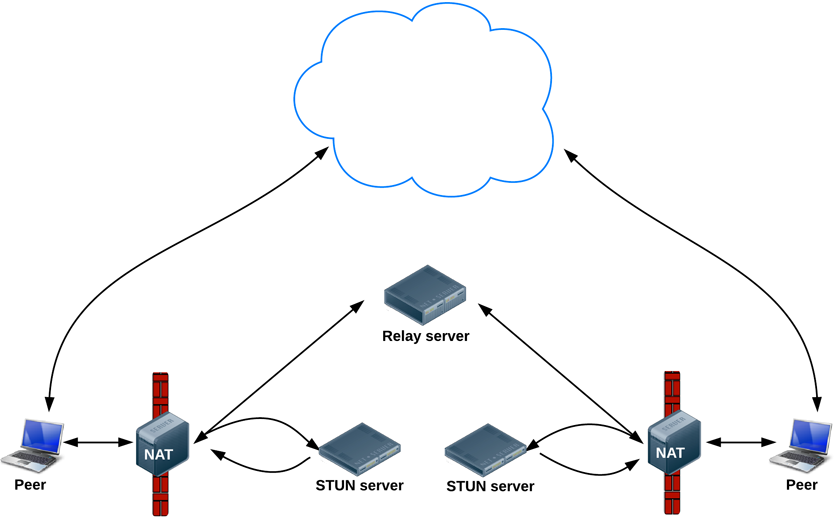
\includegraphics[width=\textwidth,height=0.25\paperheight,keepaspectratio
]{figures/ICE}
\caption{The different ways for ICE to find network interfaces and ports \cite{WebRTCBasics:2012:Online}}
\label{fig:ICE}
\end{figure}

ICE decides between different ways of achieving a connection and chooses the one with the lowest latency\cite{WebRTCBasics:2012:Online}. At first ICE tries to connect peers cleanly through UDP and STUN (Session Traversal Utilities for NAT). STUN servers are simple, cheap to run and enables a peer behind a NAT to discover its public adress and port. When the IP-addresses are known data doesn't need to go througn the server but instead flows directly between the peers. However, if it is not possible to establish a connection ICE attempts to use TCP instead of UDP: first HTTP and then HTTPS.

\begin{figure}[htp]
\centering
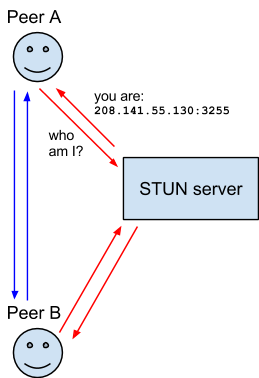
\includegraphics[width=\textwidth,height=0.2\paperheight,keepaspectratio
]{figures/webrtc-stun}
\caption{STUN servers lets peers in a private network behind firewalls discover their public IP-adresses\cite{WebRTCArchitecture:2014:Online}.}
\label{fig:WebRTC - STUN}
\end{figure}

If STUN doesn't work, probably because of firewalls and more advanced NAT systems, ICE uses cloud fallback in the form of a TURN (Traversal Using Relay NAT) server. This connection isn't peer-to-peer since the data needs to go through the server and because of this it is also slower than the previous alternatives. But it allows a connection to be made under almost any condition.

\begin{figure}[htp]
\centering
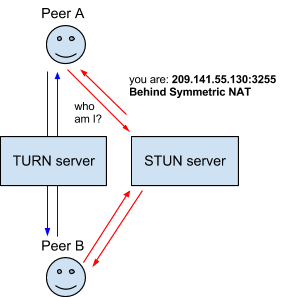
\includegraphics[width=\textwidth,height=0.2\paperheight,keepaspectratio
]{figures/webrtc-turn}
\caption{If a peer-to-peer connection cannot be made, a relay through a TURN server could be used instead. All peers then send their packets through the relay which is more costly but makes the system work\cite{WebRTCArchitecture:2014:Online}.}
\label{fig:WebRTC - TURN}
\end{figure}

\subsection{Implementation}
\label{sec:p2p}
% Niklas

% - built on top of peerjs
Rymd leverages the open source project PeerJS\footnote{http://peerjs.com}, which simplifies sending peer-to-peer data between clients. PeerJS makes use of WebRTC and is essentially split into two components: A server that acts as the signaling channel and a client side API which interacts with the server as well as other peers. The server just handles the brokering of connections, which implies that only the data necessary for negotiating a connection is sent through that point. After a connection has been setup between two clients, the server is no longer needed in order for them to communicate.

% - elaborate
Behind the scenes Peer.js handles the communication between clients and the server with the help of Websockets, but falls back to other protocols if a browser lacks support.


\section{Authentication}

% TODO Robert

\subsection{Namecoin}
A phenomenon that has been on the rise during recent years is that of cryptocurrencies such as Bitcoin \cite{CryptoCoinInsider:2014:Online}. Each participant in the Bitcoin network keeps a ledger of all transactions throughout the history of the network. In order for a transaction to be deemed valid, it needs to be included in a cryptographically signed block together with a salt by one of the nodes, with a hash that has a special format. It is this brute-force search for salts that generate these hashes that are called \emph{mining} and constitute the work done by \emph{miners} to keep the network running. As an incentive, each verified block also includes a reward to the miner that first finds it and submits it to the blockchain\cite{InternetForBeginners:2014:Online}. In effect, all transactions ever made are publicly available and tracked so that anyone can confirm their validity. This prevents forgery and double-spending of bitcoins.

Another cryptocurrency is Namecoin\cite{CryptoCoinInsider:2014:Online}. Namecoin is essentially a fork of Bitcoin with new transaction types that allows its blockchain to be utilized as a distributed key-value store. Although similar in nature to Bitcoin, its main purpose is to be used as a decentralized domain name system (DNS), rather than as a monetary currency.

With a decentralized DNS such as Namecoin, top level domains (such as \emph{.com} or \emph{.se}) can exist without being controlled by any central authority \cite{CryptoCoinInsider:2014:Online}. Also, the DNS lookup tables where domain names and their IP addresses are stored are shared in a peer-to-peer manner. The only necessary condition for these domains to be accessible is that there are participants willing to run the DNS server software. Although mainly intended to be used as a DNS, it contains several namespaces where arbitrary strings such as public cryptographic keys can be stored.

\section{Encryption}

% TODO Johannes

\section{Testing}
\label{sec:testing}
Automatic unit tests have been implemented where possible. No integration or functional tests have been written for testing larger parts of the system, due to the fast iteration of the library's interface and constant change in the implementation.
% TODO: more here?
